\documentclass{article}

\usepackage{fullpage}
\usepackage{amsmath}
\usepackage{amsfonts}
\usepackage{graphicx}
\usepackage{algorithmic}
\usepackage{xcolor}
\usepackage{framed}

\definecolor{dark_red}{rgb}{0.5,0.0,0.0}

\newcommand{\abs}[1]{\left|#1\right|}
\newcommand{\atan}{\text{atan}}
\newcommand{\rowvec}[3]{\left\langle #1, #2, #3 \right\rangle}
\newcommand{\colvec}[3]{\begin{bmatrix} #1 \\ #2 \\ #3 \end{bmatrix}}
\newcommand{\at}[1]{\left. #1 \right|}
\newcommand{\diff}[2]{\frac{d #1}{d #2}}
\newcommand{\partdiff}[2]{\frac{\partial #1}{\partial #2}}
\newcommand{\mvec}[1]{\overrightarrow{\mathbf{#1}}}
\newcommand{\pvec}[1]{\overrightarrow{#1}}
\newcommand{\dr}[1]{\textcolor{dark_red}{#1}}


\title{Double and Triple Integrals}
\date{}

\begin{document}

\maketitle



%%%%%%%%%%%%%% QUESTION 1
\section*{Question 1:}

Find the minimum and maximum values of the function:
\[f(x,y) = x + y\]
subject to the constraint:
\[x^2 + 4y^2 - 4x - 16y = -16\] 

%%%%%%%%%%%%%% SOLUTION 1
\vspace{5mm}
\dr{\textbf{Solution:}}

\dr{Let \(g(x,y) = x^2 + 4y^2 - 4x - 16y\) so \(\nabla f = \begin{bmatrix} 1 \\ 1 \end{bmatrix}\) and \(\nabla g = \begin{bmatrix} 2x - 4 \\ 8y - 16 \end{bmatrix}\). To find the candidate points for minimum and maximum, the following system must be solved: 
\[\left\{\begin{array}{c} 1 = \lambda(2x - 4) \\ 1 = \lambda(8y - 16) \\ x^2 + 4y^2 - 4x - 16y = -16 \end{array}\right.\]
The first equation can be solved to give \(\lambda = \frac{1}{2x - 4}\), but before this can be done, the scenario where \\ \(2x - 4 = 0\) must be considered. \(2x - 4 = 0 \iff x = 2\) so this condition causes the system to become: 
\(\left\{\begin{array}{c} 1 = 0 \\ 1 = \lambda(8y - 16) \\ 4 + 4y^2 - 8 - 16y = -16 \end{array}\right.\)
which is a contradiction. So we now know that \(x \neq 2\) and that \(\lambda = \frac{1}{2x - 4}\). The second equation becomes:
\[1 = \frac{8y - 16}{2x - 4} \iff 8y - 16 = 2x - 4 \iff y = (1/4)x + 3/2\]
The last equation becomes:
\begin{align*}
& x^2 + 4y^2 - 4x - 16y = -16 \\
\iff & x^2 + 4((1/4)x + 3/2)^2 - 4x - 16((1/4)x + 3/2) = -16 \\
\iff & x^2 + ((1/4)x^2 + 3x + 9) - 4x + (-4x - 24) = -16 \\
\iff & (5/4)x^2 - 5x = -1 
\iff x^2 - 4x = -4/5 
\iff (x - 2)^2 = 16/5 \\
\iff & x = 2 \pm 4/\sqrt{5}
\end{align*}
which in turn gives: \(y = (1/4)(2 \pm 4/\sqrt{5}) + 3/2 = 2 \pm 1/\sqrt{5}\) so the candidate points are \((2 + 4/\sqrt{5}, 2 + 1/\sqrt{5})\) and \((2 - 4/\sqrt{5}, 2 - 1/\sqrt{5})\). 
\begin{itemize}
\item \(f(2 + 4/\sqrt{5}, 2 + 1/\sqrt{5}) = 4 + \sqrt{5}\) (which is the maximum)
\item \(f(2 - 4/\sqrt{5}, 2 - 1/\sqrt{5}) = 4 - \sqrt{5}\) (which is the minimum)
\end{itemize}
}




%%%%%%%%%%%%%% QUESTION 2
\section*{Question 2:}

Find the minimum and maximum values of the function:
\[f(x,y) = 2x + y\]
subject to the constraint:
\[x^2 + y^2 - 2x - 2y = 2\]

%%%%%%%%%%%%%% SOLUTION 2
\vspace{5mm}
\dr{\textbf{Solution:}}

\dr{Let \(g(x,y) = x^2 + y^2 - 2x - 2y\) so \(\nabla f = \begin{bmatrix} 2 \\ 1 \end{bmatrix}\) and \(\nabla g = \begin{bmatrix} 2x - 2 \\ 2y - 2 \end{bmatrix}\). To find the candidate points for minimum and maximum, the following system must be solved: 
\[\left\{\begin{array}{c} 2 = \lambda(2x - 2) \\ 1 = \lambda(2y - 2) \\ x^2 + y^2 - 2x - 2y = 2 \end{array}\right.\]
The first equation can be solved to give \(\lambda = \frac{2}{2x - 2}\), but before this can be done, the scenario where \\ \(2x - 2 = 0\) must be considered. \(2x - 2 = 0 \iff x = 1\) so this condition causes the system to become: 
\(\left\{\begin{array}{c} 2 = 0 \\ 1 = \lambda(2y - 2) \\ 1 + y^2 - 2 - 2y = 2 \end{array}\right.\)
which is a contradiction. So we now know that \(x \neq 1\) and that \(\lambda = \frac{2}{2x - 2} = \frac{1}{x - 1}\). The second equation becomes:
\[1 = \frac{2y - 2}{x - 1} \iff 2y - 2 = x - 1 \iff y = (1/2)x + 1/2\]
The last equation becomes:
\begin{align*}
& x^2 + y^2 - 2x - 2y = 2 \\
\iff & x^2 + ((1/2)x + 1/2)^2 - 2x - 2((1/2)x + 1/2) = 2 \\
\iff & x^2 + ((1/4)x^2 + (1/2)x + 1/4) - 2x + (-x - 1) = 2 \\
\iff & (5/4)x^2 - (5/2)x = 11/4 
\iff x^2 - 2x = 11/5 
\iff (x - 1)^2 = 16/5 \\
\iff & x = 1 \pm 4/\sqrt{5}
\end{align*}
which in turn gives: \(y = (1/2)(1 \pm 4/\sqrt{5}) + 1/2 = 1 \pm 2/\sqrt{5}\) so the candidate points are \((1 + 4/\sqrt{5}, 1 + 2/\sqrt{5})\) and \((1 - 4/\sqrt{5}, 1 - 2/\sqrt{5})\). 
\begin{itemize}
\item \(f(1 + 4/\sqrt{5}, 1 + 2/\sqrt{5}) = 3 + 2\sqrt{5}\) (which is the maximum)
\item \(f(1 - 4/\sqrt{5}, 1 - 2/\sqrt{5}) = 3 - 2\sqrt{5}\) (which is the minimum)
\end{itemize}
}




%%%%%%%%%%%%%% QUESTION 3
\section*{Question 3:}

\begin{tabular}{cc}
\parbox{0.6\textwidth}{The leaf shaped region \(\sigma\) on the right is bounded from below by a parabola and from above by a straight line. Express \(\sigma\) as a Type I Cartesian region; a Type II Cartesian region; and a Polar region. In addition, given an arbitrary function \(f(x,y)\), or \(f(r,\theta)\) in polar coordinates, express the double integral \(\iint_{\sigma} f(x,y)dA\) as a nested (iterated) integral using each of the 3 different forms of \(\sigma\). Lastly, use all of the 3 forms to compute the double integral \(\iint_{\sigma} x dA\).}
& 
\parbox{0.4\textwidth}{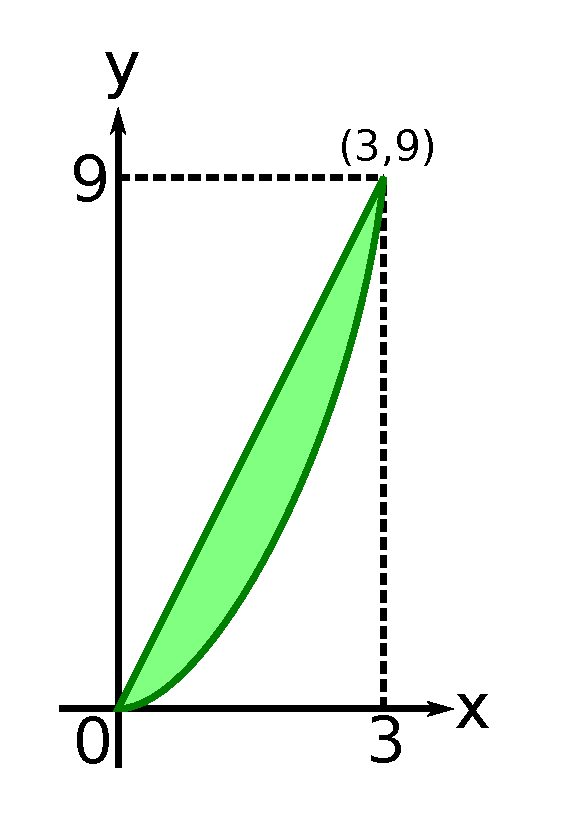
\includegraphics[height = 5cm]{Test_bench_part_3_images/Test_bench_part_3_image_5}}
\end{tabular}

%%%%%%%%%%%%%% SOLUTION 3
\vspace{5mm}
\dr{\textbf{Solution:}}

\dr{The line has the equation \(y = 3x\) which is equivalent to \(x = y/3\). The parabola has the equation \(y = x^2\) which is equivalent to \(x = \pm \sqrt{y}\). \\
The Type I formulation is:
\[\sigma = \{(x,y) | 0 \leq x \leq 3 \;\text{and}\; x^2 \leq y \leq 3x\}\]
The Type II formulation is:
\[\sigma = \{(x,y) | 0 \leq y \leq 9 \;\text{and}\; y/3 \leq x \leq \sqrt{y}\}\]
For the polar formulation, the equation \(y = x^2\) must be converted to polar coordinates: 
\begin{align*}
y = x^2 \iff & r\sin\theta = r^2\cos^2\theta 
\iff r^2 = r\frac{\sin\theta}{\cos^2\theta} \\
\iff & r = 0, \frac{\sin\theta}{\cos^2\theta}
\end{align*}
Since the parabola is tangent to the x-axis, the lower bound on \(\theta\) is \(0\). The upper bound on \(\theta\) is the counterclockwise angle that the line \(y = 3x\) makes with the positive x-axis which is \(\atan(3)\). The polar formulation of \(\sigma\) is:
\[\sigma = \{(r,\theta) | 0 \leq \theta \leq \atan(3) \;\text{and}\; 0 \leq r \leq \frac{\sin\theta}{\cos^2\theta}\}\] 
}

\dr{
The double integrals over \(\sigma\) are:
\[\iint_{\sigma} f(x,y)dA = \int_{x = 0}^3 \int_{y = x^2}^{3x} f(x,y)dydx\]
\[\iint_{\sigma} f(x,y)dA = \int_{y = 0}^9 \int_{x = y/3}^{\sqrt{y}} f(x,y)dxdy\]
\[\iint_{\sigma} f(r,\theta)dA = \int_{\theta = 0}^{\atan(3)} \int_{r = 0}^{\frac{\sin\theta}{\cos^2\theta}} f(r,\theta) \cdot r \cdot drd\theta\]
}

\dr{Evaluating \(\iint_{\sigma} x dA\) with each of the 3 forms gives:
\begin{align*}
\iint_{\sigma} x dA = & \int_{x = 0}^3 \int_{y = x^2}^{3x} x dydx 
= \int_{x = 0}^3 \at{xy}_{y = x^2}^{3x} dx 
= \int_{x = 0}^3 (3x^2 - x^3)dx 
= \at{(x^3 - \frac{1}{4}x^4)}_{x = 0}^3 \\
= & (27 - \frac{81}{4}) - 0 
= \frac{108 - 81}{4}
= \frac{27}{4}
\end{align*}
and
\begin{align*}
\iint_{\sigma} x dA = & \int_{y = 0}^9 \int_{x = y/3}^{\sqrt{y}} x dxdy 
= \int_{y = 0}^9 \at{\frac{1}{2}x^2}_{x = y/3}^{\sqrt{y}} dy 
= \int_{y = 0}^9 (\frac{1}{2}y - \frac{1}{18}y^2)dy 
= \at{(\frac{1}{4}y^2 - \frac{1}{54}y^3)}_{y = 0}^9 \\
= & (\frac{81}{4} - \frac{9^3}{6 \cdot 9}) - 0
= \frac{81}{4} - \frac{54}{4} 
= \frac{27}{4}
\end{align*}
and
\begin{align*}
\iint_{\sigma} x dA = & \iint_{\sigma} r\cos\theta dA 
= \int_{\theta = 0}^{\atan(3)} \int_{r = 0}^{\frac{\sin\theta}{\cos^2\theta}} r^2\cos\theta \cdot drd\theta 
= \int_{\theta = 0}^{\atan(3)} \at{\frac{r^3}{3}\cos\theta}_{r = 0}^{\frac{\sin\theta}{\cos^2\theta}}d\theta \\
= & \int_{\theta = 0}^{\atan(3)} \frac{\sin^3\theta}{3\cos^5\theta} d\theta 
= \int_{\theta = 0}^{\atan(3)} \frac{\cos^2\theta - 1}{3\cos^5\theta} (-\sin\theta)d\theta \\
= & \int_{\theta = 0}^{\atan(3)} \frac{1}{3}((\cos\theta)^{-3} - (\cos\theta)^{-5})(-\sin\theta)d\theta 
= \at{\frac{1}{3}(-\frac{1}{2}(\cos\theta)^{-2} + \frac{1}{4}(\cos\theta)^{-4})}_{\theta = 0}^{\atan(3)} \\
= & \frac{1}{3}(-\frac{1}{2(1/\sqrt{1 + 3^2})^2} + \frac{1}{4(1/\sqrt{1 + 3^2})^4}) - \frac{1}{3}(-\frac{1}{2} + \frac{1}{4}) \\
= & \frac{1}{3}(-5 + 25) + \frac{1}{12} 
= \frac{81}{12} 
= \frac{27}{4}
\end{align*}
It can be readily seen that all approaches give the same result.
}




%%%%%%%%%%%%%% QUESTION 4
\section*{Question 4:}

\begin{tabular}{cc}
\parbox{0.6\textwidth}{For the parabolic region \(\sigma\) on the right, express \(\sigma\) as: a Type I Cartesian region; a Type II Cartesian region; and a Polar region. In addition, given an arbitrary function \(f(x,y)\), or \(f(r,\theta)\) in polar coordinates, express the double integral \(\iint_{\sigma} f(x,y)dA\) as a nested (iterated) integral using each of the 3 different forms of \(\sigma\). Lastly, choose one of the 3 forms to compute the double integral \(\iint_{\sigma} \frac{dA}{x}\).}
& 
\parbox{0.4\textwidth}{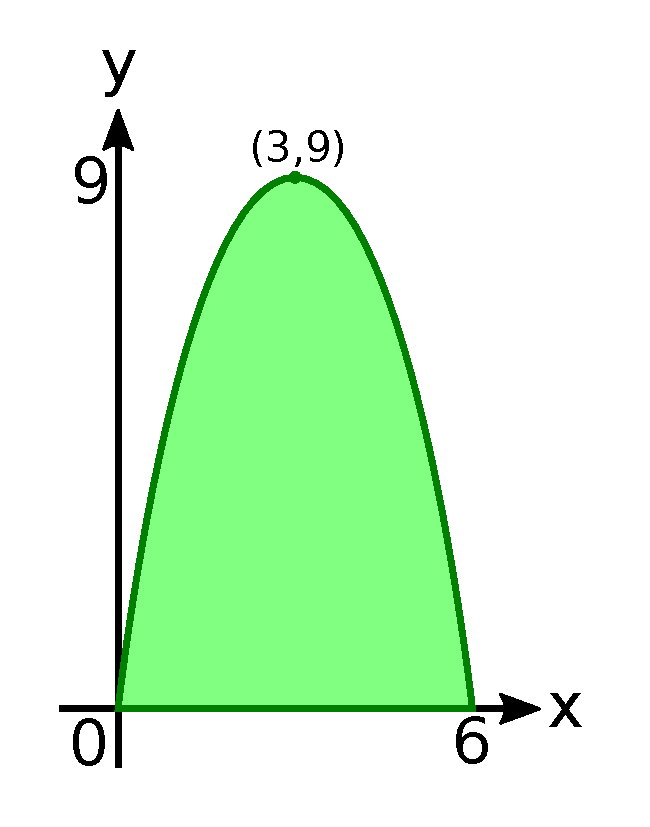
\includegraphics[height = 5cm]{Test_bench_part_3_images/Test_bench_part_3_image_1}}
\end{tabular}

%%%%%%%%%%%%%% SOLUTION 4
\vspace{5mm}
\dr{\textbf{Solution:}}

\dr{The parabola has the equation \(y = 9 - (x - 3)^2 = 6x - x^2\) which is also equivalent to \(x = 3 \pm \sqrt{9 - y}\). \\
The Type I formulation is:
\[\sigma = \{(x,y) | 0 \leq x \leq 6 \;\text{and}\; 0 \leq y \leq 6x - x^2\}\]
The Type II formulation is:
\[\sigma = \{(x,y) | 0 \leq y \leq 9 \;\text{and}\; 3 - \sqrt{9 - y} \leq x \leq 3 + \sqrt{9 - y}\}\]
For the polar formulation, the equation \(y = 6x - x^2\) must be converted to polar coordinates: 
\begin{align*}
y = 6x - x^2 \iff & r\sin\theta = 6r\cos\theta - r^2\cos^2\theta 
\iff r^2 = r\frac{6\cos\theta - \sin\theta}{\cos^2\theta} \\
\iff & r = 0, \frac{6 - \tan\theta}{\cos\theta}
\end{align*}
The lower bound on \(\theta\) is clearly \(0\). The upper bound on \(\theta\) occurs when \(\frac{6 - \tan\theta}{\cos\theta}\) becomes \(0\) after \(\theta\) increases from \(0\). This occurs when \(\theta = \atan(6)\). The polar formulation of \(\sigma\) is:
\[\sigma = \{(r,\theta) | 0 \leq \theta \leq \atan(6) \;\text{and}\; 0 \leq r \leq \frac{6 - \tan\theta}{\cos\theta}\}\] 
}

\dr{
The double integrals over \(\sigma\) are:
\[\iint_{\sigma} f(x,y)dA = \int_{x = 0}^6 \int_{y = 0}^{6x - x^2} f(x,y)dydx\]
\[\iint_{\sigma} f(x,y)dA = \int_{y = 0}^9 \int_{x = 3 - \sqrt{9 - y}}^{3 + \sqrt{9 - y}} f(x,y)dxdy\]
\[\iint_{\sigma} f(r,\theta)dA = \int_{\theta = 0}^{\atan(6)} \int_{r = 0}^{\frac{6 - \tan\theta}{\cos\theta}} f(r,\theta) \cdot r \cdot drd\theta\]
}

\dr{
The double integral \(\iint_{\sigma} \frac{dA}{x}\) is easiest to evaluate using the type I Cartesian formulation. This is determined through experimentation:
\begin{align*}
\iint_{\sigma} \frac{dA}{x} = & \int_{x = 0}^6 \int_{y = 0}^{6x - x^2} \frac{1}{x}dydx 
= \int_{x = 0}^6 \at{\frac{y}{x}}_{y = 0}^{6x - x^2}dx 
= \int_{x = 0}^6 (6 - x)dx \\
= & \at{(6x - \frac{1}{2}x^2)}_{x = 0}^6 
= (36 - 18) - 0 = 18
\end{align*}
}




%%%%%%%%%%%%%% QUESTION 5
\section*{Question 5:}

\begin{tabular}{cc}
\parbox{0.6\textwidth}{For the circular region \(\sigma\) on the right, express \(\sigma\) as a polar region, and then express the double integral \(\iint_{\sigma} f(r,\theta)dA\) as a nested integral. Lastly, evaluate the double integral \(\iint_{\sigma} \frac{\sqrt{\sin(2\theta)} \cdot dA}{r}\).} 
&
\parbox{0.4\textwidth}{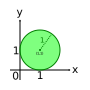
\includegraphics[width = 0.4\textwidth]{Test_bench_part_3_images/Test_bench_part_3_image_2}}
\end{tabular}

%%%%%%%%%%%%%% SOLUTION 5
\vspace{5mm}
\dr{\textbf{Solution:}}

\dr{
The circle that bounds \(\sigma\) has the Cartesian equation \((x - 1)^2 + (y - 1)^2 = 1\) which needs to converted to polar coordinates:
\begin{align*}
(x - 1)^2 + (y - 1)^2 = 1 \iff & x^2 + y^2 - 2x - 2y = -1 \\
\iff & r^2\cos^2\theta + r^2\sin^2\theta - 2r\cos\theta - 2r\sin\theta = -1 \\
\iff & r^2 - 2r(\cos\theta + \sin\theta) + 1 = 0 \\
\iff & r = \frac{2(\cos\theta + \sin\theta) \pm \sqrt{4(\cos\theta + \sin\theta)^2 - 4}}{2} \\
\iff & r = (\cos\theta + \sin\theta) \pm \sqrt{2\cos\theta\sin\theta} \\
\iff & r = (\cos\theta + \sin\theta) \pm \sqrt{\sin(2\theta)}
\end{align*}
The bound on \(\theta\) are clearly \(0\) and \(\pi/2\). Therefore:
\[\sigma = \{(r,\theta) | 0 \leq \theta \leq \pi/2 \;\text{and}\; (\cos\theta + \sin\theta) - \sqrt{\sin(2\theta)} \leq r \leq (\cos\theta + \sin\theta) + \sqrt{\sin(2\theta)}\}\]
\[\iint_{\sigma} f(r,\theta)dA = \int_{\theta = 0}^{\pi/2} \int_{r = (\cos\theta + \sin\theta) - \sqrt{\sin(2\theta)}}^{(\cos\theta + \sin\theta) + \sqrt{\sin(2\theta)}} f(r,\theta) \cdot r \cdot drd\theta\]
Lastly, 
\begin{align*}
\iint_{\sigma} \frac{\sqrt{\sin(2\theta)} \cdot dA}{r} = & \int_{\theta = 0}^{\pi/2} \int_{r = (\cos\theta + \sin\theta) - \sqrt{\sin(2\theta)}}^{(\cos\theta + \sin\theta) + \sqrt{\sin(2\theta)}} \frac{\sqrt{\sin(2\theta)}}{r} \cdot r \cdot drd\theta \\
= & \int_{\theta = 0}^{\pi/2} \at{\sqrt{\sin(2\theta)} \cdot r}_{r = (\cos\theta + \sin\theta) - \sqrt{\sin(2\theta)}}^{(\cos\theta + \sin\theta) + \sqrt{\sin(2\theta)}}d\theta \\ 
= & \int_{\theta = 0}^{\pi/2} 2\sin(2\theta) d\theta 
= \at{-\cos(2\theta)}_{\theta = 0}^{\pi/2} 
= 1 - (-1) = 2
\end{align*}
}




%%%%%%%%%%%%%% QUESTION 6
\section*{Question 6:}

Given the polar nested integral:
\[\int_{\theta = -\atan(2)}^{\pi/4}\int_{r = 0}^{\frac{2\cos\theta + \sin\theta}{\cos^2\theta}} r^2\cos\theta dr d\theta\]
Sketch the region covered by this double integral, convert it to Cartesian coordinates, and lastly evaluate the integral.

%%%%%%%%%%%%%% SOLUTION 6
\vspace{5mm}
\dr{\textbf{Solution:}}

\dr{
The domain of integration is: \(\sigma = \{(r,\theta) | -\atan(2) \leq \theta \leq \pi/4 \;\text{and}\; 0 \leq r \leq \frac{2\cos\theta + \sin\theta}{\cos^2\theta}\}\). \\
To convert this domain to Cartesian coordinates, the equation \(r = \frac{2\cos\theta + \sin\theta}{\cos^2\theta}\) must be converted to Cartesian coordinates:
\begin{align*}
r = \frac{2\cos\theta + \sin\theta}{\cos^2\theta} 
\iff & r = \frac{2(x/r) + y/r}{(x/r)^2} 
\iff 1 = \frac{2x + y}{x^2} 
\iff y = x^2 - 2x
\end{align*}
Hence \(\sigma\) is bounded by the parabola \(y = x^2 - 2x\). \\
\begin{tabular}{cc}
\parbox{0.6\textwidth}{
The lower bound of \(\theta = -\atan(2)\) results in the line \(y = x \cdot \tan(-\atan(2)) = -2x \iff y = -2x\), while the upper bound of \(\theta = \pi/4\) results in the line \(y = x \cdot \tan(\pi/4) = x \iff y = x\). 
The line \(y = -2x\) intersects the parabola when \(x^2 - 2x = -2x \iff x = 0\). This single intersection point at the origin means that this line is tangent to the parabola at the origin, and hence lies outside of the parabola. The line \(y = x\) intersects that parabola when \(x^2 - 2x = x \iff x(x - 3) = 0 \iff x = 0, 3\) so the intersection points are \((0,0)\) and \((3,3)\). The region \(\sigma\) is sketched to the right. 
} & \parbox{0.4\textwidth}{

\includegraphics[height = 5cm]{Test_bench_part_3_images/Test_bench_part_3_Solutions_image_1}
}
\end{tabular}
\(\sigma\) using the Type I Cartesian formulation is:
\[\sigma = \{(x,y) | 0 \leq x \leq 3 \;\text{and}\; x^2 - 2x \leq y \leq x\}\]
so hence:
\[\int_{\theta = -\atan(2)}^{\pi/4}\int_{r = 0}^{\frac{2\cos\theta + \sin\theta}{\cos^2\theta}} r^2\cos\theta dr d\theta
= \iint_{\sigma} r\cos\theta dA = \iint_{\sigma} x dA = 
\int_{x = 0}^3 \int_{y = x^2 - 2x}^{x} x dydx\]
Therefore:
\begin{align*}
\iint_{\sigma} x dA = & \int_{x = 0}^3 \int_{y = x^2 - 2x}^{x} x dydx 
= \int_{x = 0}^3 \at{xy}_{y = x^2 - 2x}^{x} dx 
= \int_{x = 0}^3 (3x^2 - x^3)dx \\
= & \at{(x^3 - \frac{1}{4}x^4)}_{x = 0}^3 
= (27 - \frac{81}{4}) - 0 = \frac{27}{4}
\end{align*}
}




%%%%%%%%%%%%%% QUESTION 7
\section*{Question 7:}

Given the polar nested integral:
\[\int_{\theta = 0}^{\pi/2}\int_{r = 0}^{\frac{6}{2\cos\theta + 3\sin\theta}} r^2\cos\theta dr d\theta\]
Sketch the region covered by this double integral, convert it to Cartesian coordinates, and lastly evaluate the integral.

%%%%%%%%%%%%%% SOLUTION 7
\vspace{5mm}
\dr{\textbf{Solution:}}

\dr{
The domain of integration is: \(\sigma = \{(r,\theta) | 0 \leq \theta \leq \pi/2 \;\text{and}\; 0 \leq r \leq \frac{6}{2\cos\theta + 3\sin\theta}\}\). \\
To convert this domain to Cartesian coordinates, the equation \(r = \frac{6}{2\cos\theta + 3\sin\theta}\) must be converted to Cartesian coordinates:
\begin{align*}
r = \frac{6}{2\cos\theta + 3\sin\theta} 
\iff & r = \frac{6}{2(x/r) + 3(y/r)} 
\iff 1 = \frac{6}{2x + 3y} 
\iff y = 2 - (2/3)x
\end{align*}
Hence \(\sigma\) is bounded by the line \(y = 2 - (2/3)x\). \\
\begin{tabular}{cc}
\parbox{0.6\textwidth}{
The lower bound of \(\theta = 0\) results in the line \(y = 0\), while the upper bound of \(\theta = \pi/2\) results in the line \(x = 0\). 
The line \(y = 0\) intersects the line at \((3,0)\). The line \(x = 0\) intersects the line at \((0,2)\). The region \(\sigma\) is sketched to the right. 
} & \parbox{0.4\textwidth}{
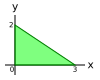
\includegraphics[height = 5cm]{Test_bench_part_3_images/Test_bench_part_3_Solutions_image_2}
}
\end{tabular}
\(\sigma\) using the Type I Cartesian formulation is:
\[\sigma = \{(x,y) | 0 \leq x \leq 3 \;\text{and}\; 0 \leq y \leq 2 - (2/3)x\}\]
so hence:
\[\int_{\theta = 0}^{\pi/2}\int_{r = 0}^{\frac{6}{2\cos\theta + 3\sin\theta}} r^2\cos\theta dr d\theta
= \iint_{\sigma} r\cos\theta dA = \iint_{\sigma} x dA = 
\int_{x = 0}^3 \int_{y = 0}^{2 - (2/3)x} x dydx\]
Therefore:
\begin{align*}
\iint_{\sigma} x dA = & \int_{x = 0}^3 \int_{y = 0}^{2 - (2/3)x} x dydx 
= \int_{x = 0}^3 \at{xy}_{y = 0}^{2 - (2/3)x} dx 
= \int_{x = 0}^3 (2x - (2/3)x^2)dx \\
= & \at{(x^2 - \frac{2}{9}x^3)}_{x = 0}^3 
= (9 - 6) - 0 = 3
\end{align*}
}




%%%%%%%%%%%%%% QUESTION 8
\section*{Question 8:}

Given the Cartesian nested integral:
\[\int_{x = -2}^2 \int_{y = 0}^{\sqrt{4-x^2}} y\sqrt{x^2 + y^2} \cdot dydx\]
Evaluate this integral directly, and then convert this integral to polar coordinates and evaluate that integral to demonstrate that you get the same result.

%%%%%%%%%%%%%% SOLUTION 8
\vspace{5mm}
\dr{\textbf{Solution:}}

\dr{
Evaluating this integral directly gives:
\begin{align*}
& \int_{x = -2}^2 \int_{y = 0}^{\sqrt{4-x^2}} y\sqrt{x^2 + y^2} \cdot dydx 
= \int_{x = -2}^2 \at{\frac{1}{3}(x^2 + y^2)^{3/2}}_{y = 0}^{\sqrt{4-x^2}} dx \\
= & \int_{x = -2}^2 (\frac{8}{3} - \frac{1}{3}\abs{x}^3) dx 
= \int_{x = -2}^0 (\frac{8}{3} - \frac{1}{3}(-x)^3) dx + \int_{x = 0}^2 (\frac{8}{3} - \frac{1}{3}x^3) dx \\
= & \int_{x = -2}^0 (\frac{8}{3} + \frac{1}{3}x^3) dx + \int_{x = 0}^2 (\frac{8}{3} - \frac{1}{3}x^3) dx
= \at{(\frac{8}{3}x + \frac{1}{12}x^4)}_{x = -2}^0 + \at{(\frac{8}{3}x - \frac{1}{12}x^4)}_{x = 0}^2 \\
= & (0 - (-\frac{16}{3} + \frac{4}{3})) + ((\frac{16}{3} - \frac{4}{3}) - 0) 
= \frac{12}{3} + \frac{12}{3} 
= 8
\end{align*}
}

\dr{
The domain of integration is: \(\sigma = \{(x,y) | -2 \leq x \leq 2 \;\text{and}\; 0 \leq y \leq \sqrt{4 - x^2}\}\). \\
To convert this domain to polar coordinates, the equation \(y = \sqrt{4 - x^2}\) must be converted to polar coordinates:
\begin{align*}
y = \sqrt{4 - x^2} 
\iff & r\sin\theta = \sqrt{4 - r^2\cos^2\theta} \\
\implies & r^2\sin^2\theta = 4 - r^2\cos^2\theta 
\iff r^2 = 4 
\iff r = 2
\end{align*}
Therefore \(\sigma\) is bounded by the circle \(r = 2\). \\
\begin{tabular}{cc}
\parbox{0.6\textwidth}{
The bounds of \(-2\) and \(2\) on \(x\) correspond to the left and right extremes of the circle and have no impact on the circle's interior. In addition, the lower bound of \(y = 0\) confines \(\sigma\) to the semicircle above the \(x\)-axis. The region \(\sigma\) is sketched on the right.
} & 
\parbox{0.4\textwidth}{
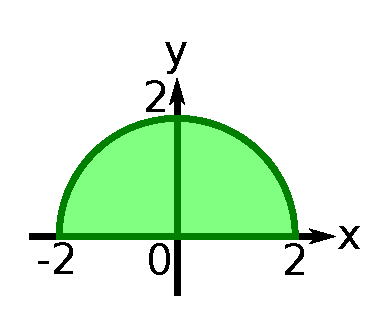
\includegraphics[height = 5cm]{Test_bench_part_3_images/Test_bench_part_3_Solutions_image_3}
}
\end{tabular}
\(\sigma\) using the polar formulation is: 
\[\sigma = \{(r,\theta) | 0 \leq \theta \leq \pi \;\text{and}\; 0 \leq r \leq 2\}\]
so hence:
\[\int_{x = -2}^2 \int_{y = 0}^{\sqrt{4-x^2}} y\sqrt{x^2 + y^2} \cdot dydx 
= \iint_{\sigma} y\sqrt{x^2 + y^2} \cdot dA
= \iint_{\sigma} r^2\sin\theta \cdot dA 
= \int_{\theta = 0}^{\pi} \int_{r = 0}^2 r^3\sin\theta \cdot drd\theta\]
Therefore:
\begin{align*}
\iint_{\sigma} r^2\sin\theta \cdot dA 
= & \int_{\theta = 0}^{\pi} \int_{r = 0}^2 r^3\sin\theta \cdot drd\theta 
= \int_{\theta = 0}^{\pi} \at{\frac{1}{4}r^4 \sin\theta}_{r = 0}^2 d\theta 
= \int_{\theta = 0}^{\pi} 4\sin\theta d\theta \\
= & \at{-4\cos\theta}_{\theta = 0}^{\pi}
= 4 - (-4) 
= 8
\end{align*}
Both formulations of the double integral give the same value of \(8\) as expected. 
}




%%%%%%%%%%%%%% QUESTION 9
\section*{Question 9:}

Compute the volume between the two surfaces \(z_1(r,\theta) = \sqrt{R^2 - r^2}\) and \(z_2(r,\theta) = -\sqrt{R^2 - r^2}\) over the region \(\sigma = \{(r,\theta)|0 \leq \theta \leq 2\pi \;\text{and}\; 0 \leq r \leq R\}\) where \(R > 0\) is a fixed constant. What is the significance of this volume?

%%%%%%%%%%%%%% SOLUTION 9
\vspace{5mm}
\dr{\textbf{Solution:}}

\dr{
\(z_1(r,\theta) \geq z_2(r,\theta)\) for all \((r,\theta) \in \sigma\). The volume between the two surfaces is:
\begin{align*}
V = & \iint_{\sigma} (z_1(r,\theta) - z_2(r,\theta))dA 
= \iint_{\sigma} 2\sqrt{R^2 - r^2}dA 
= \int_{\theta = 0}^{2\pi} \int_{r = 0}^R 2\sqrt{R^2 - r^2} \cdot r \cdot drd\theta \\
= & \int_{\theta = 0}^{2\pi} \at{-\frac{2}{3}(R^2 - r^2)^{3/2}}_{r = 0}^Rd\theta 
= \int_{\theta = 0}^{2\pi} \frac{2}{3}R^3 d\theta 
= \at{\frac{2}{3}R^3\theta}_{\theta = 0}^{2\pi} 
=\frac{4}{3}\pi R^3 
\end{align*}
This is the volume of a sphere of radius \(R\), which is exactly the shape of the volume sandwiched between surfaces \(z_1(r,\theta)\) and \(z_2(r,\theta)\).
}




%%%%%%%%%%%%%% QUESTION 10
\section*{Question 10:}

Given the volume \(\Omega = \{(x,y,z)|0 \leq x \leq 1 \;\text{and}\; 0 \leq y \leq 2x \;\text{and}\; 0 \leq z \leq 3y\}\), compute the triple integral: 
\[\iiint_{\Omega} xyz dV\]

%%%%%%%%%%%%%% SOLUTION 10
\vspace{5mm}
\dr{\textbf{Solution:}}

\dr{
The triple integral is the three-fold nested integral:
\begin{align*}
\iiint_{\Omega} xyz dV = & \int_{x = 0}^1 \int_{y = 0}^{2x} \int_{z = 0}^{3y} xyz \cdot dzdydx 
= \int_{x = 0}^1 \int_{y = 0}^{2x} \at{\frac{1}{2}xyz^2}_{z = 0}^{3y} dydx 
= \int_{x = 0}^1 \int_{y = 0}^{2x} \frac{9}{2}xy^3 dydx \\
= & \int_{x = 0}^1 \at{\frac{9}{8}xy^4}_{y = 0}^{2x} dx 
= \int_{x = 0}^1 18x^5 dx 
= \at{3x^6}_{x = 0}^1 
= 3
\end{align*}
}




%%%%%%%%%%%%%% QUESTION 11
\section*{Question 11:}

\begin{tabular}{cc}
\parbox{0.6\textwidth}{For the tetrahedron \(\Omega\) on the right, compute the center of mass assuming a uniform mass density \(m\). The center of mass is the weighted average position \(\rowvec{x}{y}{z}\) of the points in \(\Omega\) where the ``weight" assigned to each point is the density: \[\mathbf{r}_{\text{CM}} = \frac{\iiint_{\Omega} m\rowvec{x}{y}{z}dV}{\iiint_{\Omega} mdV} = \frac{\iiint_{\Omega} \rowvec{x}{y}{z}dV}{\iiint_{\Omega} dV}\]} 
&
\parbox{0.4\textwidth}{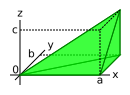
\includegraphics[width = 0.4\textwidth]{Test_bench_part_3_images/Test_bench_part_3_image_4}}
\end{tabular}

%%%%%%%%%%%%%% SOLUTION 11
\vspace{5mm}
\dr{\textbf{Solution:}}

\dr{The region \(\Omega\) is 
\[\Omega = \{(x,y,z) | 0 \leq x \leq a \;\text{and}\; 0 \leq y \leq \frac{b}{a}x \;\text{and}\; 0 \leq z \leq \frac{c}{b}y\}\]
}

\dr{The total volume of \(\Omega\) is:
\begin{align*}
\iiint_{\Omega} dV = & \int_{x = 0}^a \int_{y = 0}^{\frac{b}{a}x} \int_{z = 0}^{\frac{c}{b}y} dzdydx 
= \int_{x = 0}^a \int_{y = 0}^{\frac{b}{a}x} \at{z}_{z = 0}^{\frac{c}{b}y}dydx 
= \int_{x = 0}^a \int_{y = 0}^{\frac{b}{a}x} \frac{c}{b}ydydx \\
= & \int_{x = 0}^a \at{\frac{c}{2b}y^2}_{y = 0}^{\frac{b}{a}x}dx 
= \int_{x = 0}^a \frac{bc}{2a^2}x^2dx 
= \at{\frac{bc}{6a^2}x^3}_{x = 0}^a
= \frac{abc}{6}
\end{align*}
}

\dr{The total position in \(\Omega\) is:
\begin{align*}
\iiint_{\Omega} \colvec{x}{y}{z}dV = & \int_{x = 0}^a \int_{y = 0}^{\frac{b}{a}x} \int_{z = 0}^{\frac{c}{b}y} \colvec{x}{y}{z}dzdydx 
= \int_{x = 0}^a \int_{y = 0}^{\frac{b}{a}x} \at{\colvec{xz}{yz}{(1/2)z^2}}_{z = 0}^{\frac{c}{b}y}dydx \\
= & \int_{x = 0}^a \int_{y = 0}^{\frac{b}{a}x} \colvec{(c/b)xy}{(c/b)y^2}{(c^2/(2b^2))y^2}dydx 
= \int_{x = 0}^a \at{\colvec{(c/(2b))xy^2}{(c/(3b))y^3}{(c^2/(6b^2))y^3}}_{y = 0}^{\frac{b}{a}x}dx \\
= & \int_{x = 0}^a \colvec{((bc)/(2a^2))x^3}{((b^2c)/(3a^3))x^3}{((bc^2)/(6a^3))x^3}dx 
= \at{\colvec{((bc)/(8a^2))x^4}{((b^2c)/(12a^3))x^4}{((bc^2)/(24a^3))x^4}}_{x = 0}^a 
= \colvec{(a^2bc)/8}{(ab^2c)/12}{(abc^2)/24}
\end{align*}
}

\dr{
Therefore:
\[\mathbf{r}_{\text{CM}} = \frac{\iiint_{\Omega} \rowvec{x}{y}{z}dV}{\iiint_{\Omega} dV} = \colvec{(3/4)a}{(1/2)b}{(1/4)c}\]
}

%\dr{The region \(\Omega\) is 
%\[\Omega = \{(x,y,x) | 0 \leq x \leq a \;\text{and}\; 0 \leq y \leq b - \frac{b}{a}x \;\text{and}\; 0 \leq z \leq c - \frac{c}{a}x - \frac{c}{b}y\}\]
%}
%
%\dr{The total volume of \(\Omega\) is:
%\begin{align*}
%\iiint_{\Omega} dV = & \int_{x = 0}^a \int_{y = 0}^{b - \frac{b}{a}x} \int_{z = 0}^{c - \frac{c}{a}x - \frac{c}{b}y} dzdydx 
%= \int_{x = 0}^a \int_{y = 0}^{b - \frac{b}{a}x} \at{z}_{z = 0}^{c - \frac{c}{a}x - \frac{c}{b}y}dydx \\
%= & \int_{x = 0}^a \int_{y = 0}^{b - \frac{b}{a}x} (c - \frac{c}{a}x - \frac{c}{b}y)dydx 
%= \int_{x = 0}^a \at{(cy - \frac{c}{a}xy - \frac{c}{2b}y^2)}_{y = 0}^{b - \frac{b}{a}x}dx \\
%= & \int_{x = 0}^a (c(b - \frac{b}{a}x) - \frac{c}{a}x(b - \frac{b}{a}x) - \frac{c}{2b}(b^2 - \frac{2b^2}{a}x + \frac{b^2}{a^2}x^2))dx \\
%= & \int_{x = 0}^a ((bc - \frac{bc}{a}x) + (-\frac{bc}{a}x + \frac{bc}{a^2}x^2) + (-\frac{bc}{2} + \frac{bc}{a}x - \frac{bc}{2a^2}x^2))dx \\
%= & \int_{x = 0}^a (\frac{bc}{2} - \frac{bc}{a}x + \frac{bc}{2a^2}x^2)dx 
%= \at{(\frac{bc}{2}x - \frac{bc}{2a}x^2 + \frac{bc}{6a^2}x^3)}_{x = 0}^a
%= \frac{abc}{6}
%\end{align*}
%}
%
%\dr{The total position in \(\Omega\) is:
%\begin{align*}
%\iiint_{\Omega} \colvec{x}{y}{z}dV = & \int_{x = 0}^a \int_{y = 0}^{b - \frac{b}{a}x} \int_{z = 0}^{c - \frac{c}{a}x - \frac{c}{b}y} \colvec{x}{y}{z}dzdydx 
%= \int_{x = 0}^a \int_{y = 0}^{b - \frac{b}{a}x} \at{\colvec{xz}{yz}{(1/2)z^2}}_{z = 0}^{c - \frac{c}{a}x - \frac{c}{b}y}dydx \\
%= & \int_{x = 0}^a \int_{y = 0}^{b - \frac{b}{a}x} \colvec{cx - (c/a)x^2 - (c/b)xy}{cy - (c/a)xy - (c/b)y^2}{(c^2/(2a^2))x^2 + (c^2/(ab))xy + (c^2/(2b^2))y^2 - (c^2/a)x - (c^2/b)y + c^2/2}dydx 
%\\
%= & \int_{x = 0}^a \at{\begin{bmatrix}
%cxy - (c/a)x^2y - (c/(2b))xy^2 \\
%(c/2)y^2 - (c/(2a))xy^2 - (c/(3b))y^3 \\
%(c^2/(2a^2))x^2y + (c^2/(2ab))xy^2 + (c^2/(6b^2))y^3 ... \\
%\quad\quad ... - (c^2/a)xy - (c^2/(2b))y^2 + (c^2/2)y\end{bmatrix}}_{y = 0}^{b - \frac{b}{a}x}dx 
%\\
%= & \int_{x = 0}^a \begin{bmatrix}
%(bcx - ((bc)/a)x^2) + (-((bc)/a)x^2 + ((bc)/a^2)x^3) ... \\
%\quad\quad ... + () \\
%(c/2)y^2 - (c/(2a))xy^2 - (c/(3b))y^3 \\
%(c^2/(2a^2))x^2y + (c^2/(2ab))xy^2 + (c^2/(6b^2))y^3 ... \\
%\quad\quad ... - (c^2/a)xy - (c^2/(2b))y^2 + (c^2/2)y\end{bmatrix}dx \\
%\end{align*}
%}



\end{document}









